\chapter{Introducción}
\label{cap:introduccion}

\section{Antecedentes y motivación}
\label{intro:motivacion}

Los desastres naturales en Chile han sido frecuentes en los últimos años. Sólo por mencionar algunos de los más recientes: la erupción del volcán Chaitén (Mayo, 2008), el terremoto en Tocopilla (Noviembre, 2007), el terremoto en Concepción (2010), el incendio de las Torres del Paine (Diciembre, 2011), el incendio en Valparaíso (Abril, 2014), la erupción del volcán Villarrica (Marzo, 2015), los aluviones en el norte (Marzo, 2015), entre otros. Dependiendo de las características de la emergencia, surgen en la población diversos tipos de necesidades: alimentos, agua, luz eléctrica, refugio, rescate o comunicación. Muchas veces éstas pueden no ser detectadas por las autoridades al menos, no de forma expedita, lo que resulta perjudicial beneficioso para las personas que intentan sobrellevar de la mejor manera posible la crisis cuando se ve involucrada una necesidad básica, como la falta de agua, donde la vida de los afectados puede verse comprometida. El problema descrito no es sólo para las autoridades \cite{ChatoSurvey}, señalan que el comportamiento humano, ante crisis como éstas no es de quedarse esperando por ayuda o huir en pánico, sino de intentan tomar decisiones rápidas en base a la información que conocen. Esto quiere decir que existe gente dispuesta a ayudar, aun siendo ellos los mismos afectados; pero no siempre disponen de la información necesaria para saber dónde apuntar sus esfuerzos. Será útil, dado lo anterior, tener algún medio que concentre las necesidades que pueda tener una población dentro del país para acudir en su auxilio, posterior a la ocurrencia de una emergencia catastrófica como las mencionadas anteriormente.

Los académicos del FONDEF IDeA de la Universidad de Santiago de Chile, se han adjudicado fondos para el desarrollo de un proyecto de dos años de duración; el cual consiste en el desarrollo de una plataforma de \textit{streaming} a escala nacional, enfocada en el procesamiento de datos en caso de crisis. Esta plataforma hará uso de la información generada por los usuarios en redes sociales como fuente de datos. Se espera que esta plataforma proporcione herramientas para que cualquier persona pueda desarrollar nuevas aplicaciones permitiendo atender las diversas problemáticas que puedan existir cuando el país se enfrente a catástrofes. Para ayudar a difundir la plataforma se requiere construir tres aplicaciones: una que apoye la coordinación de voluntarios, la segunda que difunda noticias y mensajes y, finalmente, una que permita detectar necesidades de la población; todas ellas al presentarse escenarios de catástrofes naturales.

En particular, para este trabajo, se ataca el problema de la detección de necesidades de la población y servir de apoyo para la construcción de la plataforma de \textit{streaming}, en relación a qué operadores se han de construir y cómo ha de estructurarse el sistema para operar sobre datos nacionales.

\section{Descripción del problema}
\label{intro:problema}

El problema que aboda esta memoria es el hacer uso de la información generada por la población por medio de \textit{Twitter} para que, en caso de alguna emergencia de carácter nacional, pueda prestarse apoyo, en tiempo real, a las autoridades encargadas de la toma de decisiones, por ejemplo, dándoles a conocer en qué lugar en particular se requiere asistir a la población con un determinado tipo de ayuda según la necesidad que se presente. ¿Cómo puede usarse la información disponible en \textit{Twitter} para que, en casos de emergencia, ésta sea útil para ir en directo beneficio de la población en la que se generó satisfaciendo la necesidad específica que presentan?

\section{Solución propuesta}
\label{intro:solucion}

Se propone una aplicación, que al ocurrir un escenario de desastre que recoje constantemente, en tiempo real, publicaciones desde \textit{Twitter} y analice si corresponde o no a una necesidad existente en el conjunto de necesidades detectables y, en casos afirmativos, mostrarlas durante un intervalo de tiempo sobre un mapa geográfico del país haciendo uso de los metadatos asociados al tweet, en el caso en que se encuentren disponibles o hacer uso del contenido para inferir sus ubicaciones si es posible.

Como se mencionó, se espera que la aplicación esté expuesta a grandes cantidades de información, pues recibe directamente desde el \textit{stream} de \textit{Twitter}, por ello se aprovechan las capacidades de \textit{Apache Storm}, para ser capáz de procesar esta información en tiempo real para llevar a cabo la clasificación de cada entrada. A medida que los datos se clasifiquen, éstos se posicionan en el mapa, haciendo uso de Google Maps, para ser visualizados´con un icono correspondiente a su categoría particular por el usuario final del sistema.

La clasificación de los datos de entrada se está dada por la evaluación realizada por un modelo de clasificador bayesiano, éste categoriza estos datos según su contenido en siete posibles categorías.

\section{Objetivos y alcance del proyecto}
\label{intro:objetivos}

\subsection{Objetivo general}
	Construir un sistema escalable para la detección de necesidades de la población en tiempo real para escenarios de desastre natural haciendo uso de \textit{Twitter}.

\subsection{Objetivos específicos}
\begin{enumerate}
\item	Implementar un método encargado de la recolección de tweets generados dentro del territorio nacional haciendo uso de la API pública de Twitter.
\item	Especificar la taxonomía de las necesidades que serán detectadas.
\item	Diseñar e implementar el clasificador de necesidades.
\item	Definir de los elementos de procesamiento para la construcción del sistema capaz de trabajar los datos obtenidos a gran escala.
\item	Implementar una arquitectura escalable que soporte la aplicación.
\item	Evaluar la aplicación bajo condiciones de alto tráfico como es el caso de una emergencia nacional.
\end{enumerate}

\subsection{Alcances}
\label{subsec:alcances}

Se utilizan las publicaciones de \textit{Twitter} para llevar a cabo el procesamiento de la información y no se considera, en el marco de este trabajo, el uso de una red social alternativa, no porque no sea posible, sino que con el motivo de acotar el problema.

Las necesidades que la aplicación detecta no son una lista exhaustiva de las posibles existentes, sino de un subconjunto que se ha considerado más importante en el equipo de trabajo del proyecto FONDEF IDeA. De esta forma se logra acotar el problema reduciendo la cantidad de categorías y permitir una mayor precisión en la clasificación (trabajos similares han bordeado una precisión entre el sesenta y ochenta por ciento, pero estos resultados van de la mano con la cantidad de datos utilizados para entrenar), entendiendo la precisión como la relación de elementos clasificados correctamente sobre el total.

Se considera para la construcción del clasificador un subconjunto de un \textit{dataset} de cuatro millones setecientos mil \textit{tweets} recogidos desde \textit{Twitter} correspondientes al terremoto ocurrido el 2010 en Chile. Este conjunto de datos contiene mensajes en distintos idiomas y ha sido filtrada llegando a aproximadamente un millón y medio de tweets, utilizado por \cite{}, para la construcción de su aplicación sobre rumores en \textit{Twitter}. De aquel conjunto se obtendrá un subconjunto para realizar el etiquetado y ser usado como datos de entrenamiento. 

\section{Metodologías y herramientas utilizadas}
\label{intro:metodologia}

\subsection{Metodología}
\label{subsec:MetodologiaDetalle}

Para la realización de este trabajo se utilizan dos metodologías, en esta sección se ambas son definidas.

\subsubsection*{Programación Extrema}
\label{subsubsec:XP}

La Programación Extrema (\textit{Extreme Programming}, XP desde ahora en adelante), comenzó como un proyecto el 6 de Marzo de 1996. Es uno de los procesos ágiles más populares y ha sido provado exitosamente en compañias e industrias de todos los tamaños. \cite{XP}.

Su éxito se debe a que hace especial hincapié en la satisfacción del cliente por sobre la entrega de todo lo el software posible.

Aporta cinco formas escenciales para mejorar el proceso de desarrollo de software: Comunicación, simplicidad, retroalimentación, respeto y coraje: Constantemente se comunica al equipo de desarrollo con el cliente. Se intenta mantener el diseño lo más simple y sencillo posible. Se obtiene retroalimentación desde las pruebas desde el día uno. Se les entrega el software al cliente lo más pronto posible con los cambios solicitados. El éxito depende, en gran medida, del respeto y comunicación de los miembros del equipo y los clientes. Implementando XP el equipo puede responder a los cambios sin temor.

La metodología implementa unas simples reglas de trabajo, las que se dividen en cinco grandes áreas las que se detallarán a continuación.

\begin{enumerate}
\item Planeación:
	\begin{itemize}
	\item Se escriben Historias de usuario. 
	\item Se crea un plan de \textit{releases}.
	\item Se planifican liberaciones pequeñas y frecuentes.
	\item Se divide el proyecto en iteraciones.
	\item Al comienzo de cada iteración se planea cómo será.
	\end{itemize}
\item Manejo:
	\begin{itemize}
	\item Se le da al equipo una área de trabajo.
	\item Se realizan reunione del tipo \textit{stand up meeting} a díario.
	\item Se mide la velocidad del proyecto. 
	\item Se mueven a las personas de sus puestos (para que todo el equipo pueda trabajar en todo).
	\item Se solucionan problemas que instroduzcan quiebres en la metodología.
	\end{itemize}
\item Diseño:
	\begin{itemize}
	\item Simplicidad. El mejor diseño es el más simple.
	\item Se crean \textit{spikes} para reducir el riesgo.
	\item No se agregan funcionalidades antes de tiempo.
	\item Hacer uso de técnicas de \textit{refactoring}, cada vez que sea posible.
	\end{itemize}
\item Implementación:
	\begin{itemize}
	\item El cliente siempre está disponible. 
	\item El código debe ser escrito bajo estándares. 
	\item Se hace uso de \textit{Test Driven Development }(TDD).
	\item Todo el código debe hacerse haciendo uso de \textit{pair programming}.
	\item Sólo una pareja integra código a la vez.
	\item Integración a menudo.
	\item Se cuenta con un equipo dedicado a la integración.
	\item El código es de todos.
	\end{itemize}
\item Prueba:
	\begin{itemize}
	\item Todo el código debe tener pruebas unitarias.
	\item Todas las pruebas deben ser pasadas antes de una liberación.
	\item Cuando se encuentra un \textit{bug}, se crean pruebas.
	\item Los \textit{test} de aceptación se corren a menudo y sus resultados son publicados.
	\end{itemize}
\end{enumerate}

Éstas reglas por si solas pueden carecer de sentido, pero se apoyan en los \textbf{valores} que la metodología quiere entregar y que fueron mencionadas anteriormente, pero ahora son detalladas:

\begin{itemize}
\item Simplicidad: Se hace lo que se solicitó, pero no más. Ésto maximiza el valor entregado dado una fecha límite. Nuestras metas se alcanzan por medio de pequeños pasos para mitigar errores tan pronto ocurran. Se crea algo de lo que se esté orgullosos y lo se mantiene en el tiempo a costos razonables.
\item Comunicación: Todos somos partes de un equipo y nos comunicamos cara a cara a diario. Se trabaja juntos en todo: desde la toma de requerimientos hasta la implementación. Se crea la mejor solución posible al problema.
\item Retroalimentación: Cada iteración es completada seriamente entregando \textit{software} funcional. Mostraremos nuestro \textit{software} a menudo y prontamente para luego escuchar y aplicar los cambios solicitados. Se habla de nuestro proyecto y se adapta nuestro proceso a el, no al revéz.
\item Respeto: Todos dan y reciben el respeto que merecen como miembros del equipo. Todos contribuyen con valor así sea simple entusiasmo. Los desarrolladores respetan la experiencia del cliente y viceversa. 
\item Coraje: Se dice la verdad sobre el progreso y nuestras estimaciones. No se documentan excusas por si se falla, pues se planea tener éxito. No tenemos porque no trabajamos solos. Nos adaptaremos a los cambio cuando ocurran.
\end{itemize}

El proceso de XP puede puede ser aprecido en la Figura \ref{fig:procesoXP}.

\begin{figure}[H]
	\centering
	\captionsetup{justification=centering}
	\includegraphics[scale=0.6]{images/flowChartXP.png}
	\caption[Diagrama de flujo de Programación Extrema.]{Diagrama de flujo de Programación Extrema.\\Fuente: \cite{XP}}
	\label{fig:procesoXP}
\end{figure}

\subsubsection*{\textit{Knowledge Discovery in Databases} (KDD)}
\label{subsubsec:kdd}

Es definido por \cite{KDDFayyad} como "El proceso no trivial de identificar patrones válidos, nuevos, potencialmente útiles y en ultima instancia comprensible en los datos", surge de la necesidad de manejar grandes cantidades de datos e involucra simultaneamente varias disciplinas de investigación tales como el aprendizaje automático, la estadística, inteligencia artificial, sistemas de gestión de bases de datos, sistemas de apoyo a la toma de decisiones, entre otras.

Si bien puede variar el usuario, quien es aquel que determina el domino de la aplicación, es decir, cómo se utilizan los datos, el proceso generalmente considera las siguientes etapas:

\begin{enumerate}
\item Selección de datos: Consiste en buscar el objetivo y las herramientas del proceso de minería, identificando los datos que han de ser extraídos, buscando atributos apropiados de entrada y la información de salida para representar la tarea. Esto quiere decir, primero se debe tener en cuenta lo que se sabe, lo que se quiere obtener y cuáles son los datos que nos facilitarán esa información para poder llegar a nuestra meta, antes de comenzar el proceso como tal.
\item Limpieza de datos: En este paso se limpian los atributos sucios, incluyendo datos incompletos, el ruido y datos inconsistentes. Estos datos sucios, en algunos casos, deben ser eliminados, pues pueden contribuir a un análisis inexacto y resultados incorrectos.
\item Integración de datos: Combina datos de múltiples procedencias incluyendo múltiples bases de datos, que pueden tener diferentes contenidos y formatos.
\item Transformación de datos: Consiste en modificaciones sintácticas llevadas a cabo sobre los datos sin que suponga un cambio en la técnica de minería aplicada. Tiene dos caras, por un lado existen ventajas en el sentido de mejorar la interpretación de las reglas descubiertas y reduce el tiempo de ejecución, por el otro puede llevar a la pérdida de información.
\item Reducción de datos: Reducción del tamaño de los datos, encontrando características más significativas dependiendo del objetivo del proceso.
\item Minería de datos: Consiste en la búsqueda de patrones de interés que puedan expresarse como un modelo o dependencia de los datos. Se ha de de especificar un criterio de preferencia para seleccionar un modelo de un conjunto de posibles modelos. Además se ha de especificar la estrategia de búsqueda (algoritmo), a utilizar.
\item Evaluación de los patrones: Se identifican patrones interesantes que representan conocimiento utilizando diferentes técnicas incluyendo análisis estadísticos y lenguajes de consulta.
\item Interpretación de resultados: Consiste en entender resultados de análisis y sus implicaciones y puede llevar a regresar a algunos pasos anteriores.
\end{enumerate}

La representacíón del proceso descrito por la metodología KDD puede verse esquematizado en la Figura \ref{fig:procesoKDD}.

\begin{figure}[H]
	\centering
	\captionsetup{justification=centering}
	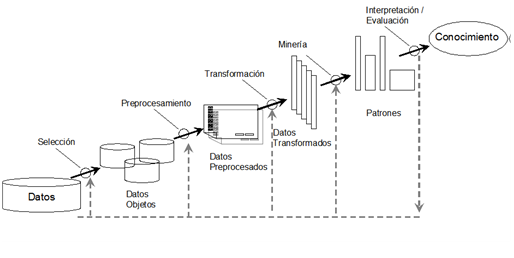
\includegraphics[scale=1]{images/kdd.png}
	\caption[Proceso KDD.]{Proceso KDD.\\Fuente: \cite{KDDFigure}}
	\label{fig:procesoKDD}
\end{figure}

\subsection{Herramientas de desarrollo}
\label{subsec:HerrDesarrollo}

A continuación se presentan las herramientas, tanto de \textit{software} como de \textit{hardware} utilizadas para la contrucción del sistema de detección de necesidades.

Se ha se utilizado diversas herramientas de software para la construcción de la aplicación, éstas son descritas a continuación haciendo especial énfasis en aquellas de gran importancia dentr del desarrollo del proyecto

\subsubsection*{Apache Storm}
\label{subsubsec:ApacheStorm}

Apache Storm es un sistema de computación en tiempo real de código abierto. Simplifica el problema de flujos (\textit{streams}), de datos sin que estos tengan fin.

Es escalable, tolerante a fallos y garantiza que toda la información será procesada. Presenta \textit{Benchmarks} que señalan que por nodo es capaz de procesar más de un millón de tuplas por segundo.

Se compone principalmente de dos partes. La primera es denominada \textit{Spout} y es la encargada de recoger el flujo de datos de entrada. La segunda es denominada \textit{Bolt} y es la encargada de la transformación o procesado de los datos.

Oficialmente es representado como puede verse en la Figura \ref{fig:stormBeLike}. donde los \textit{Spouts} son representados simulando ser llaves de agua desde donde fluyen los datos al sistema y los \textit{Bolts} como rayos donde se procesa el flujo.

\begin{figure}[H]
	\centering
	\captionsetup{justification=centering}
	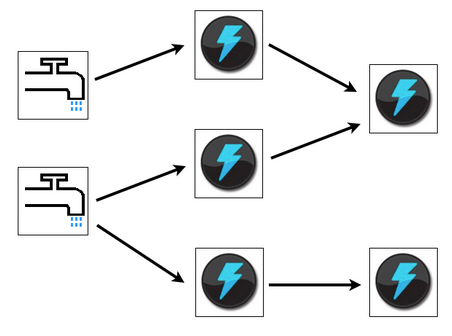
\includegraphics[scale=0.6]{images/stormBeLike.png}
	\caption[Representación del funcionamiento de Apache Storm.]{Representación del funcionamiento de Apache Storm.\\Fuente: \cite{StormFigure}}
	\label{fig:stormBeLike}
\end{figure}

Uno de los puntos fuertes que tiene este sistema es que al crear una topología donde se instancian \textit{Bolts} y \textit{Spouts}, Storm se encarga de escalar el sistema distribuyendo los elementos en sus componentes.

Al trabajar con \textit{Apache Storm}, como ya se ha descrito, se han de construir dos elementos: \textit{spout} y \textit{bolt}. Éstos elementos se construyen realizando una herencia desde \textit{BaseRichSpout}, para el caso de \textit{spout} e implementando \textit{IRichBolt} para los \textit{bolt}..

\begin{figure}[H]
	\centering
	\captionsetup{justification=centering}
	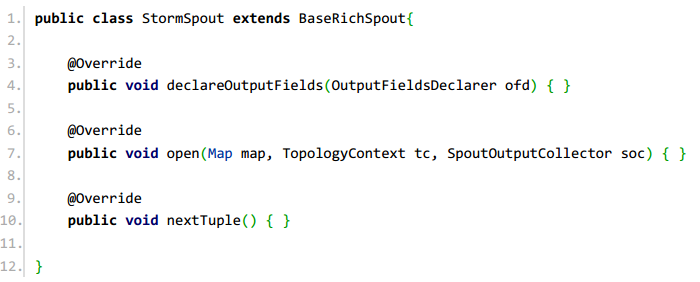
\includegraphics[scale=0.8]{images/SpoutBase.png}
	\caption[Construcción de un Spout.]{Construcción de un Spout.\\Fuente: Elaboración Propia, (2016)}
	\label{fig:spoutbase}
\end{figure}

En la figura \ref{fig:spoutbase} muestra la base para la implementación de un \textit{spout}. Cuenta con tres métodos:

\begin{itemize}
\item \textit{declareOutputFields}: declara nombres para las etiquetas que tiene el objeto emitido.
\item \textit{open}: Inicializa todos los elementos utilizados en el spout.
\item \textit{nextTuple}: es llamado desde storm al recibir una nueva tupla para realizar una tarea.
\end{itemize}	

\begin{figure}[H]
	\centering
	\captionsetup{justification=centering}
	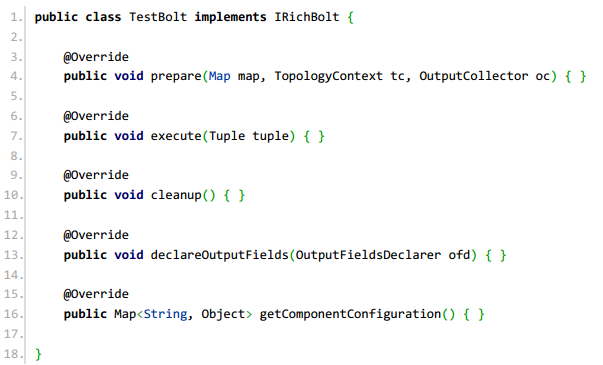
\includegraphics[scale=0.8]{images/BoltBase.png}
	\caption[Construcción de un Bolt.]{Construcción de un Bolt.\\Fuente: Elaboración Propia, (2016)}
	\label{fig:boltbase}
\end{figure}

La figura \ref{fig:boltbase} presenta la base para la implementación de un \textit{bolt}. Sus métodos se explican a continuación:

\begin{itemize}
\item \textit{prepare}: Similar al método \textit{open} para los \textit{spout}, realiza la misma función.
\item \textit{execute}: Cumple la misma función que el método \textit{nextTuple}.
\item \textit{cleanup}: Al finalizar una topología se llama este método para cerrar el \textit{bolt}.
\item \textit{declareOutputFields}: declara nombres para las etiquetas que tiene el objeto emitido.
\item \textit{getComponentConfiguration}: Usado al querer cambiar una configuración del sistema.
\end{itemize}

\textit{Spout} y \textit{bolts} se unen para dar origen a una Topología. Una topología de Storm es similar a un grafo, donde cada nodo se encarga de procesar una determinada información y le pasa el testigo al siguiente nodo. Está compuesta por \textit{Spouts} y \textit{Bolts}. \cite{Storm}.

Se refiere a la forma en la que se van a compartir los datos entre los componentes. Como modelo de datos, Storm utiliza tuplas que son listas de valores con un nombre específico. El valor puede ser cualquier tipo, para ello se ha de implementar un serializador. \cite{Storm}.

\begin{itemize}
\item Shuffle grouping: Storm decide de forma \textit{round robin} la tarea a la que se va a enviar la tupla, de manera que la distribución sea equivalente entre todos los nodos.
\item Fields grouping: Se agrupan los \textit{streams} por un determinado campo de manera que se distribuyen los valores que cumplen una determinada condición a la misma tarea.
\item All grouping: El \textit{stream} pasa por todas las tareas haciendo multicast.
\item Grobal grouping: El \textit{stream} se envía al \textit{bolt} con ID más bajo.
\item None grouping: Es un \textit{Shuffle grouping} donde el orden no es importante.
\item Direct grouping: La tarea es la encargada de decidir hacia donde emitir especificando el ID del destinatario.
\item Local grouping: Se utiliza el mismo \textit{bolt} si tiene una o más tareas en el mismo proceso.
\end{itemize}

Storm puede funcionar de dos modos: Local y Cluster. El primero es útil para el desarrollo, pues ejecuta toda la topología en una única JVM, por lo que pueden realizarse fácilmente pruebas de integración, depurar código, etcétera. Este modo simula, haciendo uso de \textit{Threads}, cada nodo del Cluster. \cite{Storm}.

El modo Cluster es considerado el 'modo de producción' y es el modo donde el código es distribuido en máquinas diferentes dentro del Cluster.

La arquitectura de Storm se divide en tres componentes:
\begin{itemize}
\item Master Node: Ejecuta el demonio llamado Nimbus, el cual es responsable de distribuir el código a través del cluster. Realiza la asignación y monitorización de tareas en las distintas máquinas del cluster.
\item Worker Node: Ejecutan el demonio Supervisor, el cual se encarga de recoger y procesar los trabajos asignados en la máquina donde está corriendo. En caso de fallo de uno \textit{Worker Node}, Nimbus observa esto y redirige el trabajo a otro.
\item Zookeeper: Si bien no es un componente propio de Storm, es necesario para su funcionamiento, pues se encarga de coordinar Nimbus y Supervisor, además de mantener sus estados, pues ambos son \textit{stateless}.
\end{itemize}

\subsubsection*{MongoDB}
\label{subsubsec:mongoDB}

Base de datos no relacional (NoSQL) de código abierto escrita en C++ y está orientada al trabajo en documentos. Lo anterior quiere decir que, en lugar de guardar los datos en registros, lo hace en documentos y éstos son almacenada en una representación binaria de JSON conocida como BSON.

Una de las diferencias fundamentales con respecto a las bases de datos relacionales es que no es necesario que se siga un esquema; en una misma colección - concepto similar a una tabla en las bases de datos relacionales - pueden tener distintos esquemas.

MongoDB fue creado para brindar escalabilidad, rendimiento y disponibilidad. Puede ser utilizado en un servidor único como en múltiples. Esto se logra dado que MongoDB brinda un elevado rendimiento, tanto para lectura como para escritura, potenciando la computación en memoria.

Las consultas en MongoDB se realizan como si se tratase de Javascript entregando como parámetro un objeto JSON. Por ejemplo, dado el documento presentado en la Figura \ref{fig:MongoJsonExample}, parte de una colección llamada 'Personas' en MongoDB:

\begin{figure}[H]
	\centering
	\captionsetup{justification=centering}
	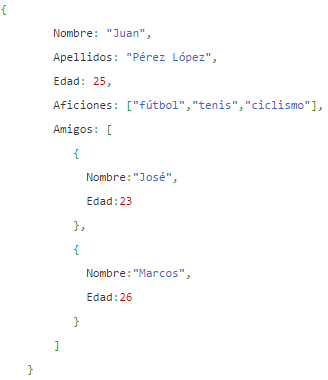
\includegraphics[scale=0.8]{images/MongoJsonExample.png}
	\caption[Documento en MongoDB.]{Documento en MongoDB.\\Fuente: Elaboración Propia, (2016)}
	\label{fig:MongoJsonExample}
\end{figure}

Una consulta para encontrar este elemento dentro de la colección se da de la forma aprecida en la Figura \ref{fig:MongoJsonQueryExample}

\begin{figure}[H]
	\centering
	\captionsetup{justification=centering}
	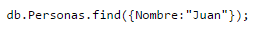
\includegraphics[scale=0.8]{images/MongoJsonQueryExample.png}
	\caption[Consulta en MongoDB.]{Consulta en MongoDB.\\Fuente: Elaboración Propia, (2016)}
	\label{fig:MongoJsonQueryExample}
\end{figure}

En pruebas realizando operaciones habituales dentro de las bases de datos \cite{MongoPerformance} demostró que el tiempo de ejecución de MongoDB, como base de datos NoSQL, aventaja significativamente a las bases de datos relacionales más populares como lo son MySQL y PostgreSQL.

\subsubsection*{Play Framework}
\label{subsubsec:playframework}

Es un \textit{framework} de código abierto para aplicaciones \textit{web} escrito en \textit{Java} y \textit{Scala}, el cual sigue el patrón de arquitectura \textit{Modelo-Vista-Controlador} (MVC). Utiliza el paradigma de diseño "Convención sobre configuración", el cual apunta a reducir la toma de decisiones que debe tomar el desarrollador sin perder flexibilidad. 

Se enfoca en la productividad a aplicaciones \textit{RESTful}.

Elimina la desventaja de desarrollo al utilizar \textit{Java} dada por el continuo ciclo de compilar-empaquetamiento-despliegue. Al detectar cambios en el código realiza inmediatamente la compilación y actualiza en la JVM sin necesidad de reiniciar el servidor.

\textit{Play} no utilizar sesiones en su funcionar, privilegiando el uso de almacenamiento \textit{offline} o el uso de peticiones \textit{Ajax} para resolver problemas del lado del cliente.

\subsubsection*{Mallet}
\label{subsubsec:mallet}

Fué desarrollada por \cite{Mallet}, en la Universidad de Massachusetts Amherst, es una herramienta de Java para el procesamiento de lenguaje natural, clasificación de documentos, \textit{clustering}, extracción de información y otras aplicaciones de aprendizaje de máquina sobre texto.

Cuenta con implementaciones de una variedad de algoritmos entre los cuales se encuentran: Naïve Bayes, Máxima entropía y árboles de decisión. Además incluye herramientas para evaluar el desempeño de clasificadores mediante el uso de métricas más utilizadas.

\subsubsection*{Otras herramientas de \textit{software}}
\label{subsubsec:herrSoft}

Además de las herramientas descritas se hace uso de las una lista de herramientas comunes para el desarrollo de proyectos de \textit{software} presentada a continuación:

\begin{itemize}
\item NetBeans (8.1), como herramienta de apoyo a la construcción de la aplicación.
\item Sublime Text 3 (Build 3103), como editor de textos.
\item MiKTex (XeLaTeX), para la escritura de la memoria.
\item PowerDesigner 16, para la elaboración de diagramas.
\item Bitbucket (Git), como repositorio de todo lo referente al proyecto (Detector de necesidades, visualizador y documento de memoria).
\item Windows 10 Home Edition (x64).
\item YourKit 1.8.0\_92 64 bits, para evaluación de \textit{performance} de la aplicación.
\item Linux Mint 17.3 (x86).
\item Oracle VirtualBox (5.0.14).
\end{itemize}

\subsubsection*{Herramientas de \textit{hardware}}
\label{subsubsec:HerrHardw}

Se hace uso del equipo del autor de este trabajo cuyas características técnicas son descritas a contunuación:
\begin{itemize}
\item Procesador Intel Core i5 2.2 Ghz.
\item 8 GB de memoria RAM.
\item 1 TB de disco duro.
\end{itemize}

\section{Organización del documento}
\label{intro:organizacion}

A continuación se presentan a grueso modo los capítulos que componen el presente documento:

El Capítulo \ref{cap:MarcTeorico}. \nameref{cap:MarcTeorico}, presenta tanto el estado de arte, correspondiente a los últimos que se ha investigado o desarrollado con respecto a los tópicos que componen éste trabajo, como una serie de definiciones detalladas para ayudar a comprender de mejor manera el problema y los elementos utilizados para su resolución.

El Capítulo \ref{cap:Requerimientos}. \nameref{cap:Requerimientos}, describe el proceso de toma de requerimientos de la aplicación. Para ello, siguiendo la metodología XP, se usan de historias de usuario y sus correspondientes criterios de aceptación.

El Capítulo \ref{cap:Diseno}. \nameref{cap:Diseno}, se presenta la arquitectura del sistema y las decisiones que llevaron a que se se optara por ésta además de describir la implementación de las aplicaciones visualizador y detector de necesidades, incluyendo los elementos que las componen y, en el caso de esta última aplicación, el porqué del uso de una topología en particular.

El Capítulo \ref{cap:experimentos}. \nameref{cap:experimentos}, describe la completitud de las historias de usuario, evalúa el nivel de replicación de los operadores del sistema y su rendimiento en una simulación de una situación real como fue el terremoto de Concepción en febrero del año 2010.

Finalmente en el Capítulo \ref{cap:conclusiones}. \nameref{cap:conclusiones}, presenta las conclusiones del trabajo realizado, el cumplimiento de objetivos tanto general como específicos, los resultados de los experimentos y trabajo futuro.